% Sweave("flsp_man.rnw")
% pdflatex flsp_man.tex
% Manual for FLsp
% Front Guff
\documentclass[a4paper]{article}
\usepackage{geometry}
\usepackage{color}
\usepackage{framed}
\usepackage{setspace}
\usepackage{amsmath}
\usepackage{hyperref}
\usepackage{cite}
\usepackage{url}
\geometry{verbose,a4paper,tmargin=2cm,bmargin=1.5cm,lmargin=2cm,rmargin=3cm}
\definecolor{shadecolor}{rgb}{0.9,0.9,0.9}
\definecolor{darkblue}{rgb}{0,0,0.5}
\setlength{\parskip}{\medskipamount}
\setlength{\parindent}{0pt}
\onehalfspacing
\hypersetup{colorlinks, urlcolor=darkblue}

% Title page
\usepackage{Sweave}
\begin{document}

\title{FLsp - a Surplus Production model in FLR}
\author{ Finlay Scott <finlay.scott@cefas.co.uk\\
Cefas, Lowestoft, UK}
\date{June 2011}
\maketitle

% Intro. What it does
\section{Introduction}

This package implements the surplus production described in Polacheck REF.
At the moment only the model including observation error is implemented.
The Pella Tomlinson shape is used (which defaults to Schaeffer)
Tested against the three data sets in the paper.
Accurate gradients and hessian are returned using automatic differentiation (implemented using ADOLC REF)

% Details of the model being implemented
\section{The Model}
Following the Polacheck paper
Assumptions:
Observation error
Only r and k are estimated
sigma and q are approximated as described in the paper
The inital biomass is k

The general equation for the biomass through time is:
\begin{equation}
B_{y+1} = B_y + g(B_y) - C_y
%R = A_{y-1} / (\alpha + \beta A_{y-1})
\end{equation}

where $B$ is the stock biomass at the start of year $y$, $C$ is the catch during the year and $g$ is surplus production as a function of biomass.

Here we implement the Pella-Tomlinson form of surplus production:
\begin{equation}
g(B) = \frac{r}{p} B(1-(B/K)^p)
\end{equation}

where $r$ is the intrinsic growth rate parameter and $K$ is the average biomass level prior to exploitation.
By default, $p$ is set to 1 making the surplus prodution formulation the same as a Schaefer model.

The biomass is related to an index of abundance:
\begin{equation}
I_y = q B_y
\end{equation}

Where I is an index of relative abundance in year $y$ and $q$ is the catchability coefficient.

Here we assume that errors are introduced through observation. The population dynamics are assumed to be deterministic and all of the error occurs in the relationship between stock biomass and the index of abundance.
It is assumed that the error is multiplicative and log-normal with a constant coefficient of variation. The estimates of the model parameters are ($B_0$, $r$, $K$ and $q$) are obtained by maximising the likeilhood function:

\begin{equation}
L = \prod exp(\hat{v}_y^2 / (2\hat{\sigma}^2_v)) / (\sqrt{2\pi}\hat{\sigma}_v)
\end{equation}

where the product is over all years for which CPUE data are available and:

\begin{align}
\hat{v}_y &= log(C/E)_y - log(\hat{C/E})_y \\
\hat{\sigma}^2_v &= \sum\hat{v}_y^2 / n
\end{align}

where $n$ is the number of data points.

The value of $q$ which maximises the likelihood is given by:

\begin{equation}
\hat{q} = exp\left(\frac{1}{n} \sum_{y} log(I_y/\hat{B_y})\right)
\end{equation}

Following Polacheck et al $B_0$ is set to $K$. This means that only two parameters need to be estimated: $r$ and $K$.
In $FLsp$ the estimation is performed using the $DEoptim$ package REF.

\section{The FLsp class}

The $FLsp$ class extends the $FLModel$ class by including slots to store the catch and index time series. Catch is represented as an $FLQuant$ and index is represented as an $FLQuants$ object. This allows multiple indices to be used (not yet implemented).

To estimate the parameters $r$ and $K$, an $FLsp$ object must be created with catch and index data. The method $fitsp()$ is then called.
Once the object has been fitted, the biomass trajectory and other variables of interest (e.g. $sigma^2$ and $\hat{q}$ can be calculated).

\section{Creating and fitting FLsp objects}

Here we show how to create and fit a surplus production model using $FLsp$. The data set is New Zealand Rock Lobster, taken from Polcheck REF.

\begin{center}
\begin{minipage}[H]{0.95\textwidth}%
\begin{shaded}%
\begin{Schunk}
\begin{Sinput}
> # Load the library
> library(FLsp)
> # Load the New Zealand Rock Lobster data set
> data(nzrl)
> # This is a dataframe with year, catch and cpue
> # Take a look at the top of it
> head(nzrl)
> # Make FLQuant objects of the catch and cpue series
> catch <- FLQuant(nzrl$catch, dimnames=list(year=nzrl$year))
> index <- FLQuant(nzrl$cpue, dimnames=list(year=nzrl$year))
> # Create the FLsp object
> nzrl <- FLsp(catch=catch,index=index)
\end{Sinput}
\end{Schunk}
\end{shaded}%
\end{minipage}
\end{center}

After creating our object we are ready to fit the parameters.

\begin{center}
\begin{minipage}[H]{0.95\textwidth}%
\begin{shaded}%
\begin{Schunk}
\begin{Sinput}
> nzrl <- fitsp(nzrl)
\end{Sinput}
\end{Schunk}
\end{shaded}%
\end{minipage}
\end{center}

The published values for this data set are:
$r$ = 0.0659, 
$K$ = 129000, 
$\hat{q}$ = 2.461e-5, 
$\sigma$ = 0.207, 
$B_{current}$ = 21150. 
These can be compared to our results by interrogating the $FLsp$ object.
\begin{center}
\begin{minipage}[H]{0.95\textwidth}%
\begin{shaded}%
\begin{Schunk}
\begin{Sinput}
> # Look at the fitted parameters
> params(nzrl)
\end{Sinput}
\begin{Soutput}
An object of class "FLPar"
params
         r          k 
4.9405e-02 1.4236e+05 
units:  NA 
\end{Soutput}
\begin{Sinput}
> # qhat
> qhat(nzrl)
\end{Sinput}
\begin{Soutput}
An object of class "FLQuant"
, , unit = unique, season = all, area = unique

     year
quant 1         
  all 2.2126e-05

units:  NA 
\end{Soutput}
\begin{Sinput}
> # sigma2
> sqrt(sigma2(nzrl))
\end{Sinput}
\begin{Soutput}
An object of class "FLQuant"
, , unit = unique, season = all, area = unique

     year
quant 1      
  all 0.20695

units:  NA 
\end{Soutput}
\begin{Sinput}
> # returns the full biomass timeseries
> biomass(nzrl)
\end{Sinput}
\begin{Soutput}
An object of class "FLQuant"
, , unit = unique, season = all, area = unique

     year
quant 1945   1946   1947   1948   1949   1950   1951   1952   1953   1954  
  all 142356 141547 140733 139893 138653 136959 134544 132075 129222 125651
     year
quant 1955   1956   1957   1958   1959   1960   1961   1962   1963   1964  
  all 120838 116732 111223 107376 104232 101593  99269  96711  93660  90689
     year
quant 1965   1966   1967   1968   1969   1970   1971   1972   1973   1974  
  all  87718  84398  80800  77744  74513  71481  68540  65818  64072  62028
     year
quant 1975   1976   1977   1978   1979   1980   1981   1982   1983   1984  
  all  60115  58843  57238  55692  53949  51554  48989  46518  43734  40846
     year
quant 1985   1986   1987   1988   1989   1990  
  all  37374  33880  30498  27182  25141  22846

units:  NA 
\end{Soutput}
\end{Schunk}
\end{shaded}%
\end{minipage}
\end{center}

It can be seen that there is good agreement between the published results and those generated with $FLsp$. The differences are likely caused by the precision of the printed data set in the Polcheck paper (REF) and the fitting method used.

\section{Testing FLsp against the other data sets}

There are two other data sets available: South Atlantic albacore ($saa$) and Northern Namibian hake ($nnh$). The above process can be repeated and the results checked against the published results.

% HIDDEN!
%\begin{center}
%\begin{minipage}[H]{0.95\textwidth}%
%\begin{shaded}%
%\end{shaded}%
%\end{minipage}
%\end{center}

TABLE OF RESULTS

\begin{tabular}{|c|c|c|c|c|c|c|}
\hline
& \multicolumn{2}{|c|}{New Zealand Rock Lobster}
& \multicolumn{2}{|c|}{South Atlantic Albacore}
& \multicolumn{2}{|c|}{Northern Namibian Hake} \\
\hline
Measure & FLsp & Published & FLsp & Published & FLsp & Published \\
\hline
r          & 0.0494 & 0.0659 &  0.3197 &  0.328 & 0.3701 & 0.379\\
K ('000 t) & 142.3564741& 129.0  &  243.3652 & 239.6  & 2823.0843 & 2772.6\\
$\sigma$   & 0.207 & 0.207  &  0.11 & 0.111 & 0.125& 0.124\\
$\hat{q}$ (x$10^4$)  &0 & 24.61&  0.264 & 26.71 &0& 4.360 \\
\hline
\end{tabular}

\section{Plotting results}
There is no generic plot for FLsp at the moment. However, it is possible to look at the fitted index and residuals using relatively simple code. For example, to plot the indices with the fitted indices you can use (see Figure~\ref{fig:fitted_index_nzrl}):

\begin{center}
\begin{minipage}[H]{0.95\textwidth}%
\begin{shaded}%
%<<fig=FALSE,eval=FALSE, quiet=TRUE,echo=TRUE,results=verbatim,keep.source=TRUE>>=
\begin{Schunk}
\begin{Sinput}
> fitted <- cbind(as.data.frame(nzrl@fitted_index),type="fitted")
> index <- cbind(as.data.frame(nzrl@index),type="index")
> index <- rbind(index,fitted)
> print(xyplot(data ~ year | qname, group=type, data=index, type="b",auto.key=TRUE))
\end{Sinput}
\end{Schunk}
\end{shaded}%
\end{minipage}
\end{center}

% Actually plot it
\begin{figure}
\begin{center}
%<<fig=TRUE,eval=TRUE, quiet=TRUE,echo=FALSE,results=hide,keep.source=FALSE>>=
%<<echo=FALSE, fig=TRUE, results=hide>>=
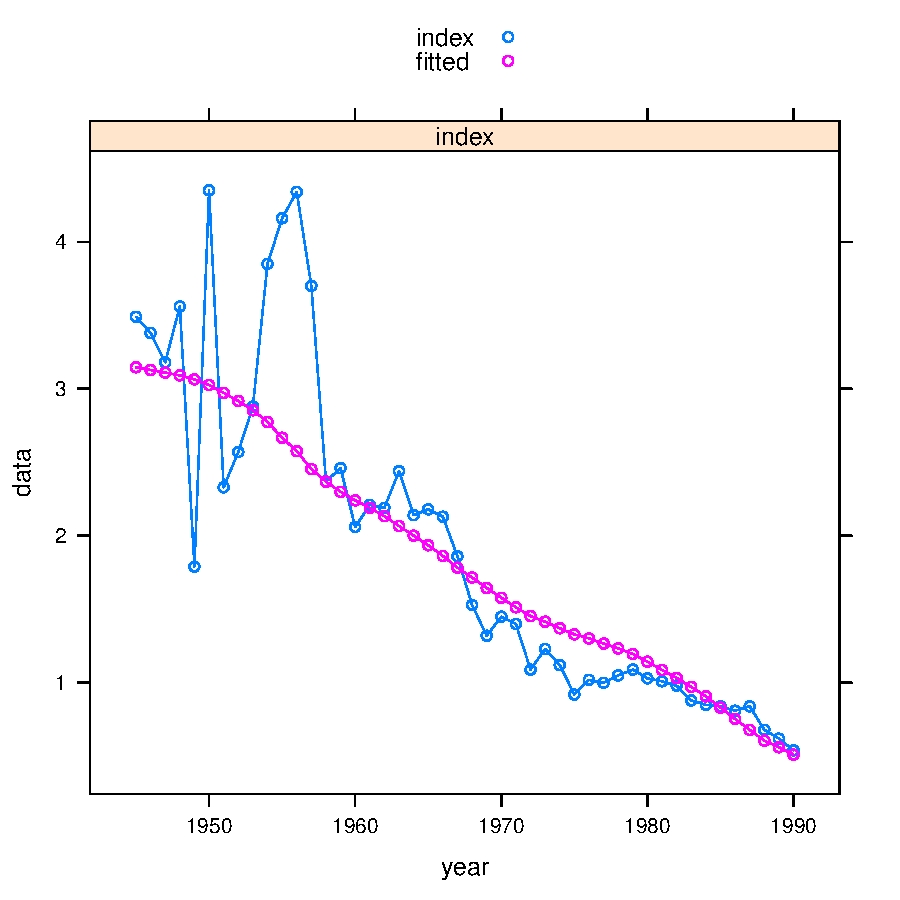
\includegraphics{flsp_man-nzrlfittedindexplot}
\end{center}
\caption{Indices and fitted indices for New Zealand rock lobster}
\label{fig:fitted_index_nzrl}
\end{figure}

To look at the residuals and put a loess function through them use (see Figure~\ref{fig:residuals_nzrl}):
\begin{center}
\begin{minipage}[H]{0.95\textwidth}%
\begin{shaded}%
%<<echo=TRUE, fig=FALSE, keep.source=TRUE,results=hide,eval=FALSE>>=
\begin{Schunk}
\begin{Sinput}
> residuals <- as.data.frame(nzrl@residuals_index)
> print(xyplot(data ~ year | qname, data = residuals, panel = function(x, 
+     y) {
+     panel.xyplot(x, y)
+     panel.loess(x, y, span = 1)
+ }))
\end{Sinput}
\end{Schunk}
\end{shaded}%
\end{minipage}
\end{center}

% Actually plot it
\begin{figure}
\begin{center}
%<<echo=FALSE, fig=TRUE, echo=FALSE>>=
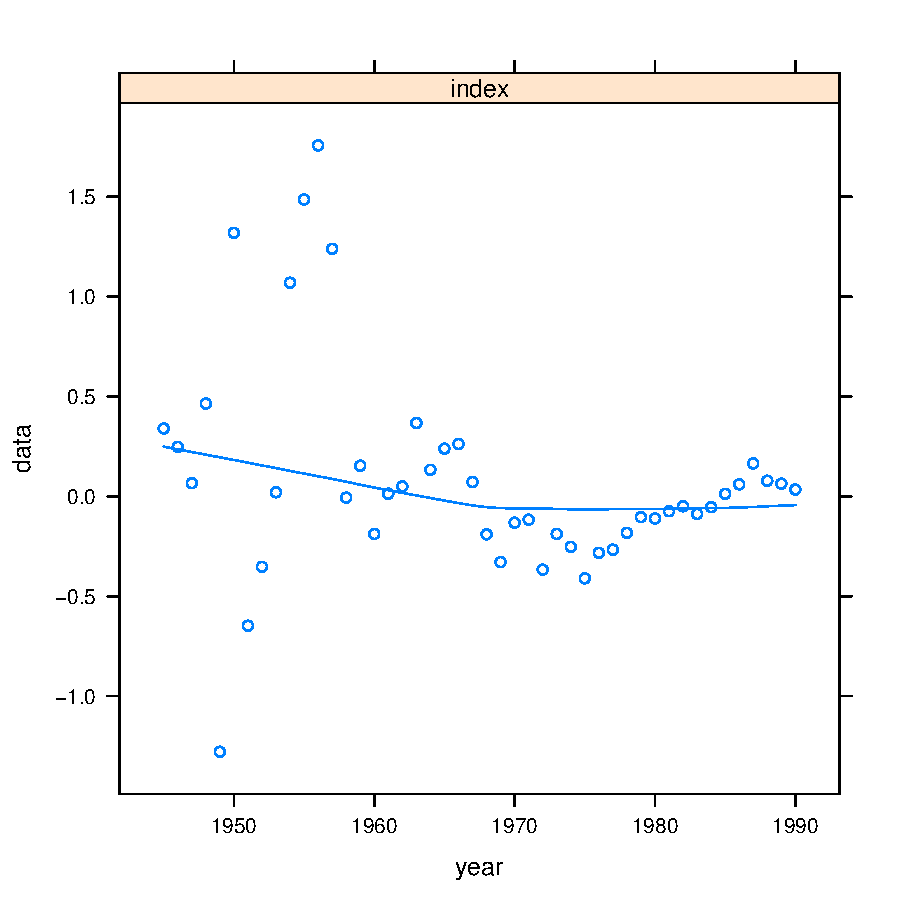
\includegraphics{flsp_man-nzrlresidplot}
\end{center}
\caption{Residuals for New Zealand rock lobster}
\label{fig:residuals_nzrl}
\end{figure}

\section{Profiling the fit}

% TO DO
% Produce table of results for all three data sets
% Plotting the results
% Something on profiling including the gradients
% MSY - plot with data
% Uncertainty and boostrapping

%\begin{center}
%\begin{minipage}[H]{0.95\textwidth}%
%\begin{shaded}%
%<<quiet=TRUE,echo=TRUE,results=hide>>=
%library(FLaspm)
%@
%\end{shaded}%
%\end{minipage}
%\end{center}



\end{document}

